\section{The Circular Polarized Alfv\'en Wave Test}

In this sample we run the circular polarized Alfv\'en wave test as descriped
on the Athena test page\footnote{
\url{http://www.astro.princeton.edu/~jstone/Athena/tests/cp-alfven-wave/cp-alfven.html}}
by Jim Stone and in the paper by Gabor Toth\footnote{
\url{http://adsabs.harvard.edu/abs/2000JCoPh.161..605T}}
(2000, J. Comp. Phys. {\bf 161}, 605).
In this setup, the density is $\rho=1$ and the pressure is $p=0.1$,
and the ratio of specific heats is $\gamma=5/3$.
In the {\sc Pencil Code}, this is achieved with $\ln\rho=s=0$ by setting
$\csz$ such that $\csz^2=\gamma p/\rho=5\times0.1/3\approx0.16666667$,
i.e., $\csz\approx0.40824829$.
Note that $\gamma=5/3$ is already the default value.
Thus, we put
\begin{verbatim}
&init_pars
  lshift_origin_lower=T
  xyz0=0., 0., 0.
  xyz1=2., 1., 0.
/
&eos_init_pars
  cs0=.40824829
/
\end{verbatim}
where {\texttt lshift\_origin\_lower=T} ensures that the lowest coordinate
index agrees with $x=y=0$.
(For a periodic mesh such as this one, the default would be shifted by
1/2 meshpoint in the positive direction.)

We consider a two-dimensional domain, $0\leq x<2$ and $0\leq y<1$.
Furthermore, velocity and magnetic field perturbations are equal to
each other, such that the components in the $xy$ plane are
\EQ
\uu_\perp=\BB_\perp=0.1\,\eee\sin\kk\cdot\xx,
\EN
where $\kk=(\pi,2\pi,0)$ and $\eee$ is a unit vector perpendicular to $\kk$.
We choose here $\eee=\zzz\times\kk/|\kk|$, where $|\kk|=\sqrt{5}\pi$.
The $z$ components of $\uu$ and $\BB$ are given by
\EQ
u_z=B_z=0.1\cos\kk\cdot\xx.
\EN
Thus, we have
\begin{equation}
\uu=\pmatrix{u_{x0}\sin(k_xx+k_yy)\cr u_{y0}\sin(k_xx+k_yy)\cr
u_{z0} \cos(k_xx+k_yy) }
\label{uu}
\end{equation}
with $u_{x0}=-0.2/\sqrt{5}\approx0.089442719$,
$u_{y0}=0.1/\sqrt{5}\approx0.044721360$, and $u_{z0}=0.1$.

The magnetic field must be specified in terms of the vector potential.
We make the ansatz
\begin{equation}
\AAA=\pmatrix{0\cr A_{y0}\sin(k_xx+k_yy)\cr A_{z0}\cos(k_xx+k_yy)},
\end{equation}
where $A_{z0}=0.1/|\kk|\approx0.014235251$ and
$A_{y0}=0.1/k_x\approx0.031830989$.
We verify that this yields
\begin{equation}
\BB=\nab\times\AAA=
\pmatrix{\partial_x\cr\partial_y\cr0}\times
\pmatrix{0\cr A_{y0}\sin(k_xx+k_yy)\cr A_{z0}\cos(k_xx+k_yy)}
=\pmatrix{-k_y A_{z0}\sin(k_xx+k_yy)\cr+k_x A_{z0}\sin(k_xx+k_yy)\cr
+k_x A_{y0} \cos(k_xx+k_yy) },
\end{equation}
in agreement with \Eq{uu}.
In the {\sc Pencil Code}, this can be accomplished by using
the initial conditions {\texttt inituu='sinwave-phase'}
and {\texttt initaa='sinwave-phase'}, i.e.,
\begin{verbatim}
&hydro_init_pars
  inituu = 'sinwave-phase'
  ampl_ux=-.089442719, kx_ux=3.1415927, ky_ux=6.2831853, kz_ux=0., phase_ux=0.
  ampl_uy=0.044721360, kx_uy=3.1415927, ky_uy=6.2831853, kz_uy=0., phase_uy=0.
  ampl_uz=0.1        , kx_uz=3.1415927, ky_uz=6.2831853, kz_uz=0., phase_uz=1.5707963
/
&magnetic_init_pars
  initaa = 'sinwave-phase'
  ampl_ax=0.0        , kx_ax=3.1415927, ky_ax=6.2831853, kz_ax=0., phase_ax=0.
  ampl_ay=0.031830989, kx_ay=3.1415927, ky_ay=6.2831853, kz_ay=0., phase_ay=0.
  ampl_az=0.014235251, kx_az=3.1415927, ky_az=6.2831853, kz_az=0., phase_az=1.5707963
/
\end{verbatim}


\begin{figure}[t!]\begin{center}
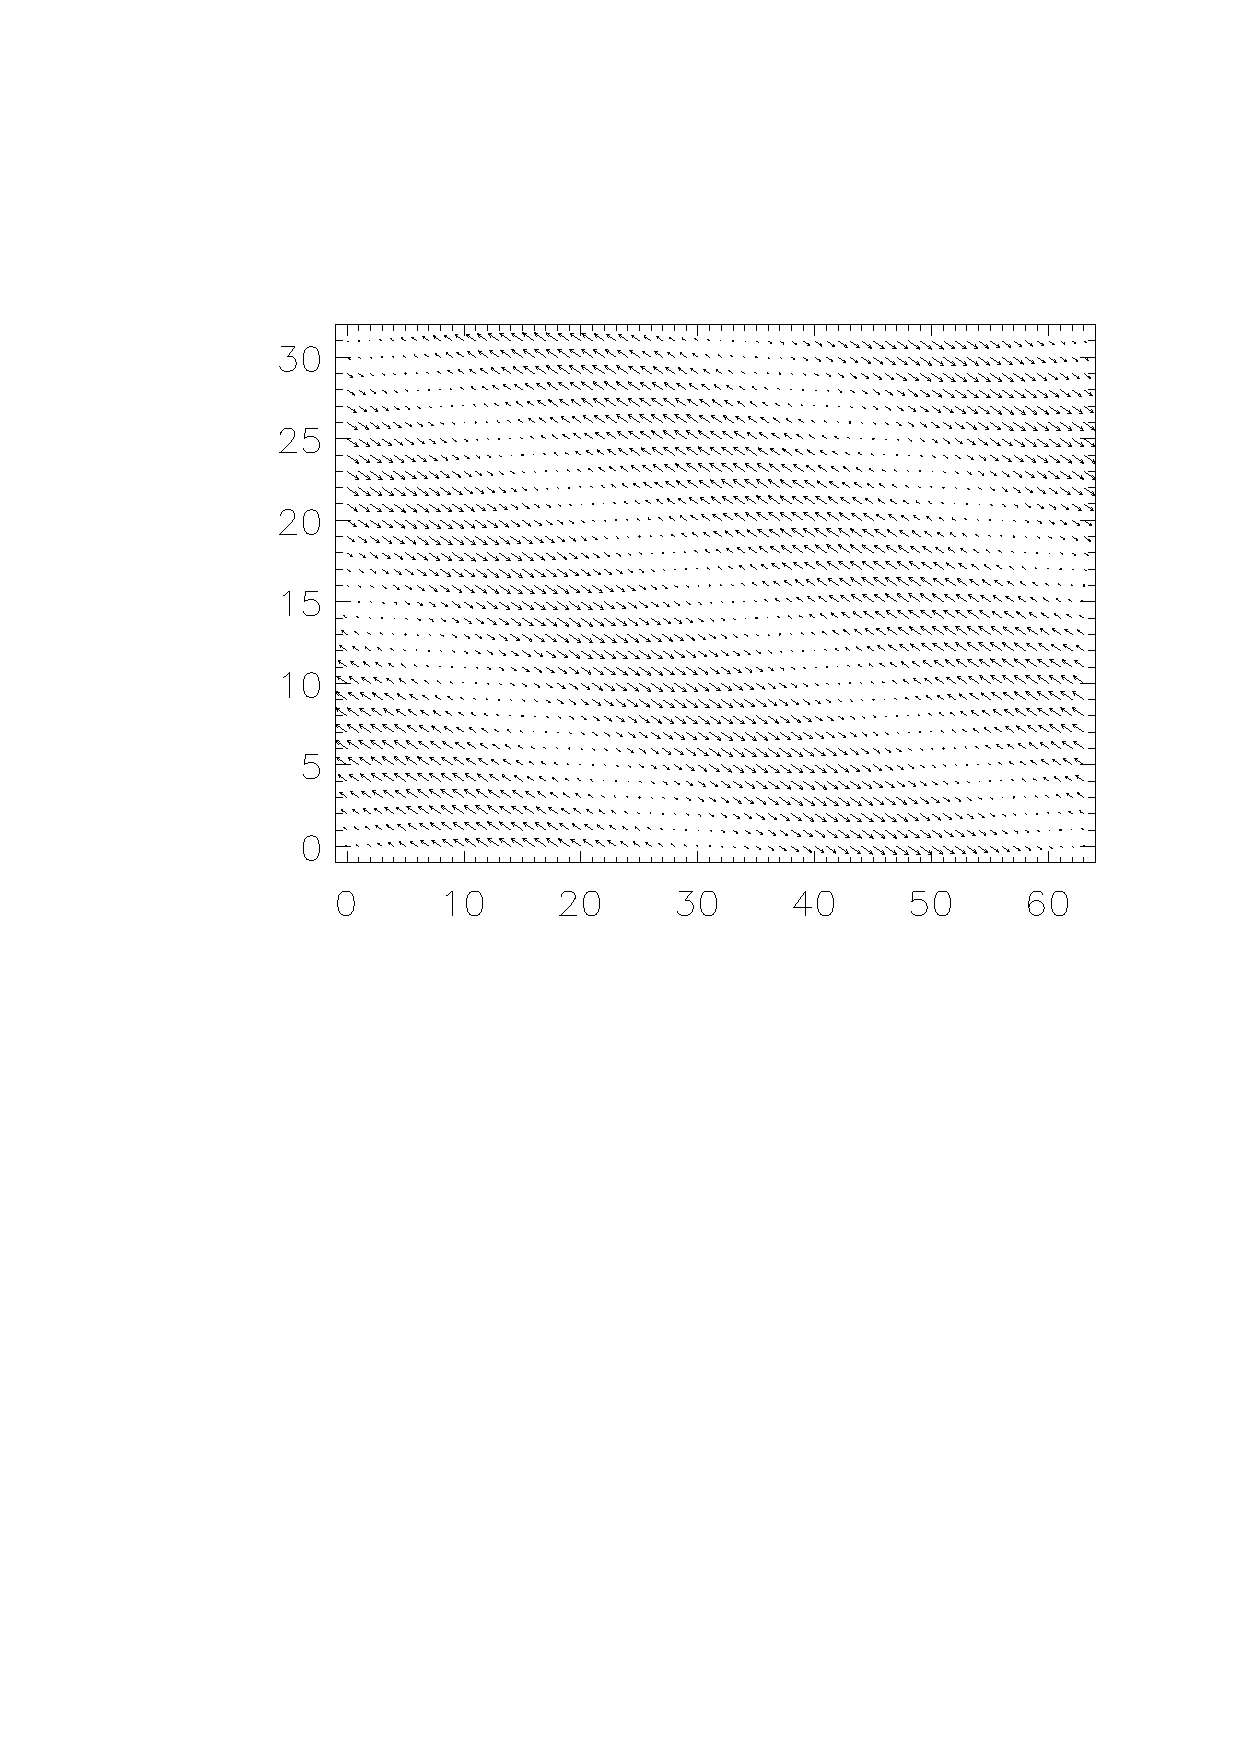
\includegraphics[width=\columnwidth]{pvar}
\end{center}\caption[]{
Perturbation
}\label{pvar}\end{figure}

%\begin{table}[htb]\caption{
%}\vspace{12pt}\centerline{\begin{tabular}{lccccccc}
%\hline
%\label{Ttimescale}\end{tabular}}\end{table}

%\begin{itemize}
%\item
%\end{itemize}
